%\begin{savequote}[8cm]
%\textlatin{Cor animalium, fundamentum e\longs t vitæ, princeps omnium, Microco\longs mi Sol, a quo omnis vegetatio dependet, vigor omnis \& robur emanat.}
%
%The heart of animals is the foundation of their life, the sovereign of everything within them, the sun of their microcosm, that upon which all growth depends, from which all power proceeds.
%  \qauthor{--- William Harvey %\cite{harvey_exercitatio_1628}
%  }
%\end{savequote}

\chapter{\label{app:appendix}Appendix}

\minitoc


\section{Accession Numbers of HipSci data} \label{app:hipsci_celllines}
The ENA Accession Numbers of the 25 biological replicates belonging to sensory neuron cell lines \cite{ipscneurons} are ERR177-: 
5544, 5551, 5552, 5554, 5594. 5595, 5596, 5598, 5600, 5601, 5631, 5634, 5637, 5638, 5640, 5641, 5643, 5644, 5684, 5685, 5686, 5687, 5688, 5689, 5693.
While all of these were used in MAJIQ Builder process (and thus contributed to the constitutive exons), only the sample with Accession Number ERR1775544 was used with the MAJIQ PSI step (and thus determined the alternatively spliced exons). 

The ENA Accession Numbers of the 20 biological replicates belonging to undifferentiated iPSC cell lines \cite{hipsci} are ERR-: 
914342, 946968, 946976, 946983, 946984, 946990, 946992, 946994, 947011, 1203463, 1243454, 1274914, 1274917, 1724696, 1724699, 1743789, 2039345, 2039336, 2278244 2278245.
Similarly, all of the above biological replicates were used in the MAJIQ Builder process. Only the samples with Accession Numbers ERR946992, ERR946984 (same cell type and donor as ERR946984, but different cell line), and ERR946968 (same cell type, but different donor) were used with MAJIQ PSI. 
%bezi1, 2 
%lexy 2
%25 biological replicates:
%ERR1775544 - 0 
%ERR1775551 - 1
%ERR1775552 - 2
%ERR1775553 - 3
%ERR1775554 - 4
%---
%ERR1775594 - 5
%ERR1775595 - 6
%ERR1775596 - 7
%ERR1775598 - 8
%ERR1775600 - 9
%ERR1775601 - 10
%--- 
%ERR1775631 - 11
%ERR1775634 - 12
%ERR1775637 - 13
%ERR1775638 - 14
%ERR1775640 - 15
%ERR1775641 - 16
%ERR1775643 - 17
%ERR1775644 - 18
%---
%ERR1775684 - 19
%ERR1775685 - 20
%ERR1775686 - 21
%ERR1775687 - 22
%ERR1775688 - 23
%ERR1775689 - 24
%ERR1775693 - 25
%
%20:
%bezi1,bezi2,eipl1,eipl2,iisa1,iisa2,kolf1,kolf2,lexy1,lexy2,rozh1,rozh2,zapk1,zapk2,aion1,aion2,aoxv1,aoxv2,bimq1,bimq2
%
%ERR914342
%
%ERR946968
%ERR946976
%ERR946983
%ERR946984
%ERR946990
%ERR946992
%ERR946994
%
%ERR947011
%
%ERR1203463
%ERR1243454
%ERR1274914
%ERR1274917
%
%ERR1724696
%ERR1724699
%ERR1743789
%
%ERR2039345
%ERR2039336
%
%ERR2278244
%ERR2278245

%unsorited, but paired: 
%ERR946992
%ERR946984
%
%ERR914342
%ERR1274917
%
%ERR1243454
%ERR946994
%
%ERR1203463
%ERR946983
%
%ERR946990
%ERR946968
%
%ERR947011
%ERR946976
%
%ERR1724696
%ERR1274914
%
%ERR1724699
%ERR1743789
%
%ERR2039345
%ERR2039336
%
%ERR2278244
%ERR2278245

\section{Additional Doc2Vec training details} \label{app:d2v}

\begin{table}[h!]
	\centering
	\begin{tabular}{ c c c  c c c} 
		\hline
		%   & configuration & & performance & \\
		Training method & DM \\
		Embedding dimensions & 100 \\
		Corpus & Human Genome GRCh38 \\
		Window size & 5\\
		Minimum count & 5\\
		Negative sampling & 5\\
		Epochs & 5\\
		
		\hline
	\end{tabular}
	\caption{Exact hyperparameters used for training Doc2Vec model.
	}
	\label{table:d2vparams}
\end{table}

The hyperparameters used during pre-training are given in Table \ref{table:d2vparams}. Except for the number of epochs, these are the same as in the baseline paper \cite{d2vsplicing}. We reduced the number of epochs from 20 to 5, as initial tests showed no performance difference between these two values. However, while \cite{d2vsplicing} don't mention what Doc2Vec implementation they use, almost all of these parameters are the same as the default parameters from the gensim library. Therefore, we believe that these parameters weren't fine-tuned very intensively. 

Two hyperparameters, not yet introduced, are mentioned in Table \ref{table:d2vparams}. Although these hyperparameters aren't very impactful when training on genomic data (as the vocabulary only consists of 64 words), we mention them for completeness:
\begin{itemize}
	\item The minimum count parameters eliminates all words which occur fewer than the minumum amount of times from the corpus. Infrequent words don't have enough examples to allow the model to learn a good representation of them. Additionally, while the individual words themselves are uncommon, the total amount of uncommong words might still be large, making it computationally expensive to keep them.
	
	\item Negative sampling \cite{w2v2} 
	is a technique to reduce the computational cost of backpropagating the gradient updates. The size of the weights in the Word2Vec or Doc2Vec can easily reach millions of learnable weights with a medium sized vocabulary: for 10,000 words in the vocabulary and 300-dimensional embedding, the matrix representing the hidden weights already has 3 million weights. This makes backpropagation expensive as all of these weights need to be updated in every step. \\
	When negative sampling is enabled, by default only the weights connected to the word the network should predict will be updated via backpropagation. Additionally, a certain number of negative samples, words which the network shouldn't predict, are randomly chosen and their weights are updated too. This dramatically reduces the computational cost of backpropagating the gradient updates, since only the weights of very few words in the vocabulary are updated. 
\end{itemize}


\section{Distribution of attention weights}

\begin{figure}[h]
	\centering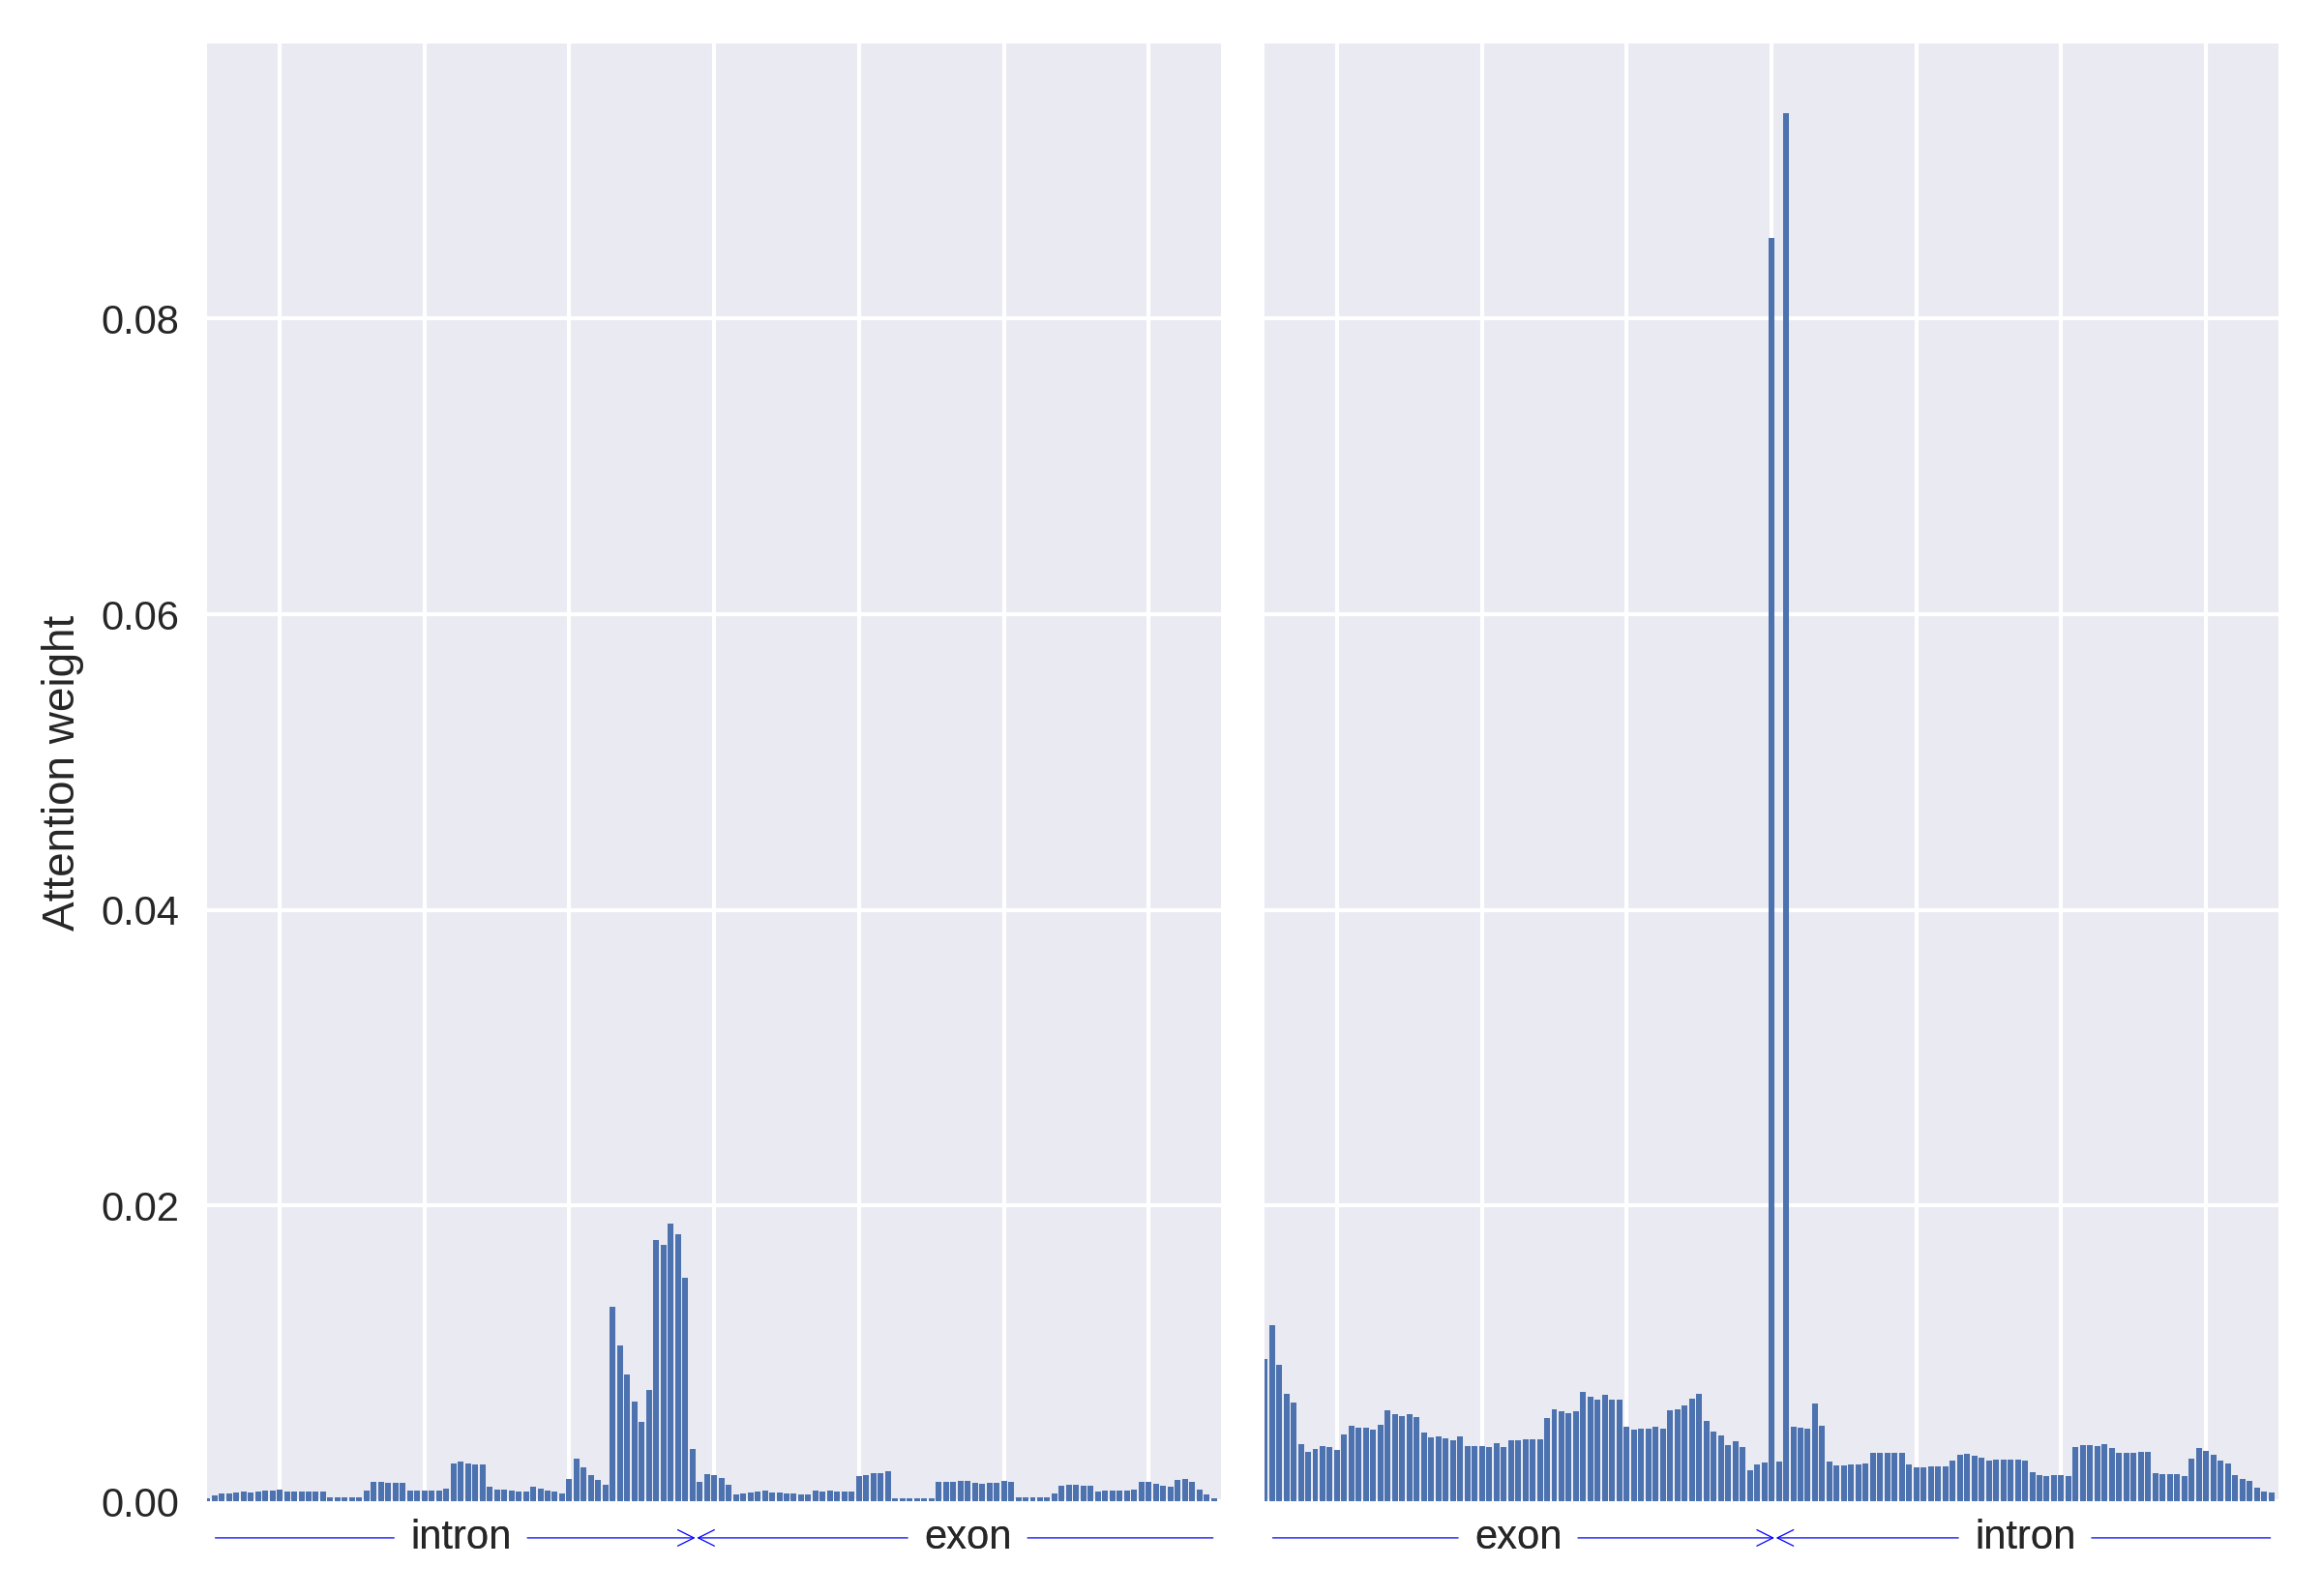
\includegraphics[width=1\textwidth]{../visualizations/ch5-results/mean_attention_barchart_not_zoomed.png}
	\caption{Mean attention weights averaged over all test samples, all cross-validation runs and all four attention heads at the end of training. }
	\label{app:mean_attn}
\end{figure}
 
%TODO do I even need to explain these if I just use the default gensim option either way?
% ---> could just explain sub-sampling too if I have time cause more text and I sound smarter
%http://mccormickml.com/2017/01/11/word2vec-tutorial-part-2-negative-sampling/

